% !TeX root = ../../main.tex
\subsection{A multi-coefficient design on real data: GSE70038}

The benchmarks so far test one coefficient at a time.  GSE70038 is the case
where the design matrix earns its place: 64,747 guides in 16 libraries from two
glioblastoma stem-cell lines and two neural stem-cell lines, with duplicate
initial and terminal samples \citep{toledo2015pkmyt1}.  The scientific target is
four cell-line-specific terminal effects estimated \emph{jointly} against one
shared initial baseline.  Four separate two-group tests cannot express that: each
would re-estimate the baseline from its own pair, discarding the other twelve
libraries that inform it.  This is therefore not a continuous-phenotype
benchmark but the multivariable one, and it is the design MAGeCKFlute documents
as the canonical multi-condition layout.

We followed the design-matrix rules in Table~5 and Box~3 of the MAGeCKFlute
protocol \citep{wang2019mageckflute}.  The first column is one for every
library; each initial library has zeros elsewhere; and each terminal library
has one in exactly one of four cell-line columns.  The same $16\times5$ matrix
was supplied to beta-binomial regression and the official MAGeCK-MLE 0.5.9.5
executable.  MAGeCK used median normalization and its Wald inference.  For the
beta-binomial result, guide effects were summarized by their within-gene
median, and directional guide $p$-values were combined by Stouffer's method.
This aggregation is an explicit comparison device, not a proposed replacement
for MAGeCK's gene model.

The ``effect rank correlation'' reported below is calculated in this analysis,
not copied from GEO or the MAGeCKFlute paper.  Separately for each terminal
coefficient, we pair all genes available from both methods.  The
beta-binomial effect is the within-gene median guide coefficient, and the
MAGeCK effect is its official MLE beta.  We assign average ranks to these two
effect vectors and take their Pearson correlation, which is exactly Spearman's
rank correlation.  The 18,077 paired effects and their ranks for every
coefficient are included with the deposited analysis output.

\begin{table}[ht]
\centering
\caption{Effect concordance between \methodswatch{barcsblue} BARCS and
\methodswatch{mageckorange} official MAGeCK-MLE on GSE70038.  Jaccard is the
overlap divided by the union of the 200 most depleted genes from each method.
Higher agreement is better; column maxima are shown in bold.}
\label{tab:gse}
\begin{tabular}{lrr}
\toprule
Terminal coefficient & Spearman effect correlation & Top-200 Jaccard\\
\midrule
GSC0131 & \textbf{0.928} & 0.550\\
GSC0827 & 0.888 & 0.533\\
NSCCB660 & 0.905 & 0.544\\
NSCU5 & 0.915 & \textbf{0.562}\\
\bottomrule
\end{tabular}
\end{table}

Concordance here is the validation rather than the finding.  The comparison is
not circular: beta-binomial regression conditions on each library total, whereas
MAGeCK uses a normalized negative-binomial count model with guide-efficiency
estimation \citep{li2015mageckvispr}.  Two models that disagree on the noise
distribution, the normalization, and the guide-efficiency treatment nevertheless
place the four coefficient vectors in the same order, with all four effect
correlations above 0.88.  That is the evidence that the model-matrix interface
recovers the intended estimand on a real screen rather than a reparameterised
approximation of it.  These correlations
measure agreement of the inferred gene ordering; they are not likelihood,
calibration, or predictive-fit statistics and therefore cannot identify a
better-fitting method.  In GSC0131, the
published convergent dependency PKMYT1 has effect $-0.987$ and FDR
$1.87\times10^{-8}$ under beta-binomial regression, versus beta $-0.786$ and
Wald FDR $4.53\times10^{-8}$ under MAGeCK-MLE.  Both also recover HEATR1,
TFAP2C, and WEE1 depletion.  Figure~\ref{fig:gse} shows the complete GSC0131
comparison; the reproducible PDF contains one page per terminal coefficient.

\begin{figure}[ht]
\centering
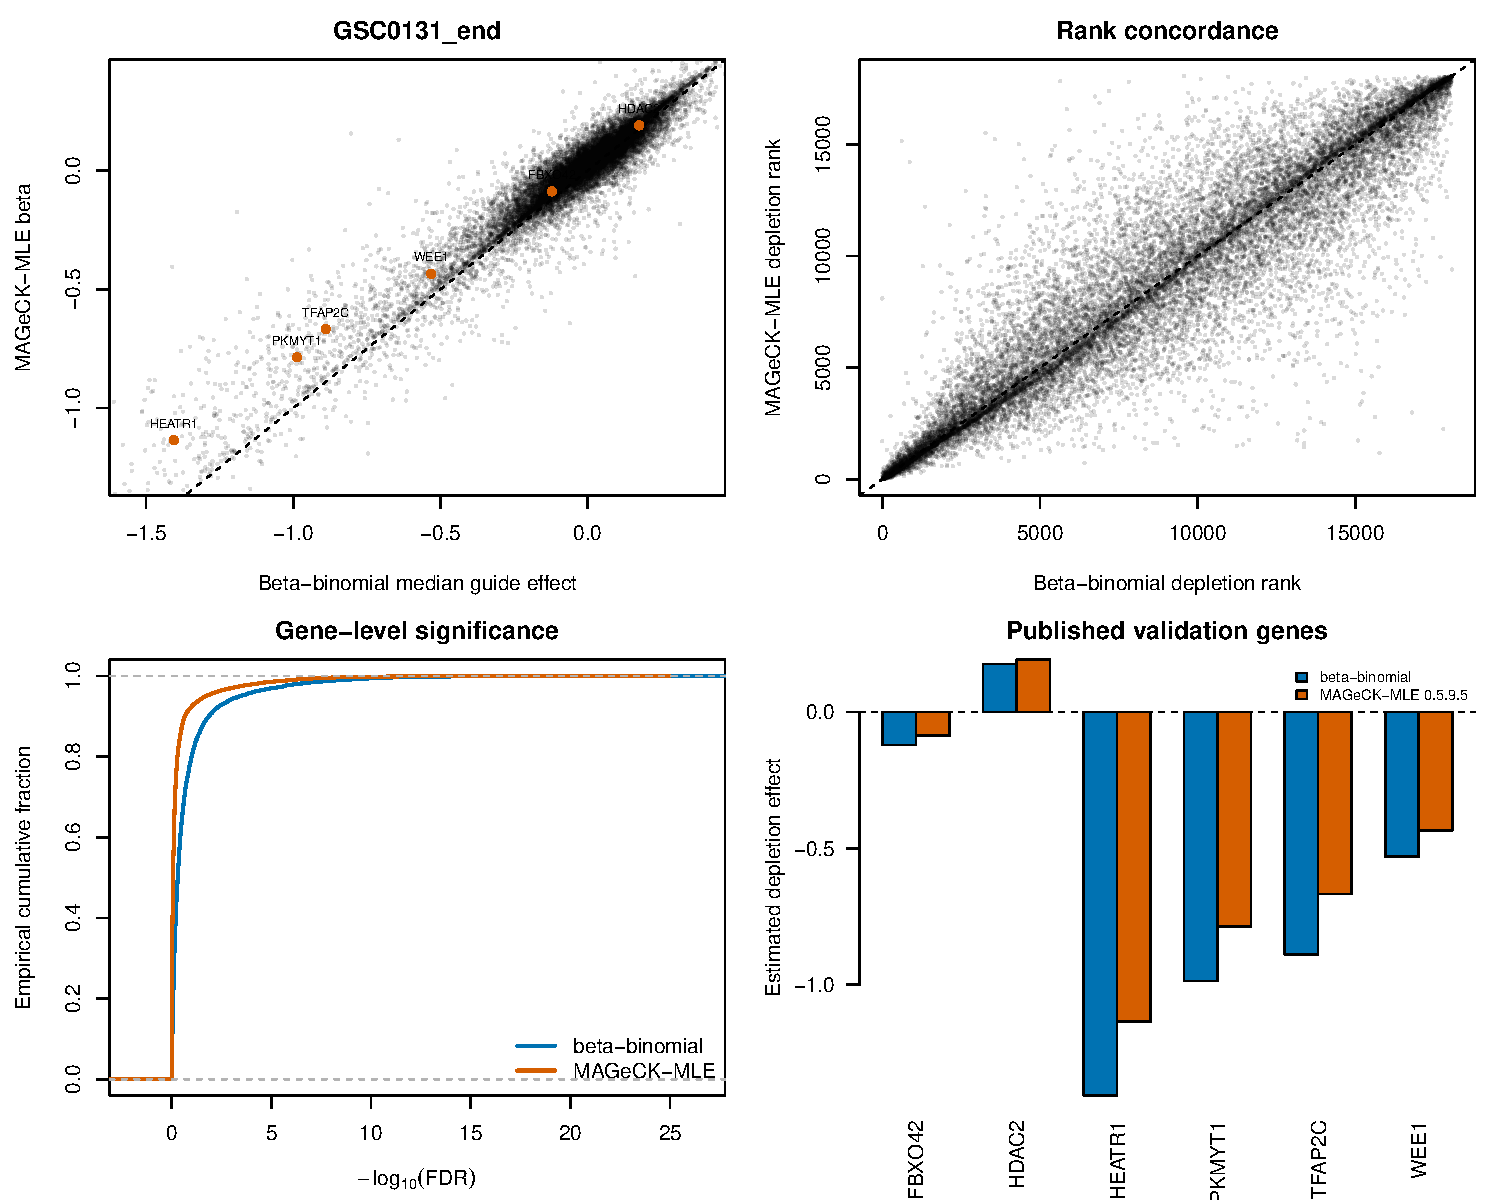
\includegraphics[width=\textwidth]{figures/gse70038_head_to_head.pdf}
\caption{GSE70038 GSC0131 head-to-head.  (A) Gene effects, with dark points
marking the prespecified genes PKMYT1, HEATR1, TFAP2C, FBXO42, HDAC2, and WEE1.
(B) Depletion-rank concordance.  (C) Gene-level FDR distributions.  (D)
Effects for the published validation genes.}
\label{fig:gse}
\end{figure}
\clearpage
